%!Mode:: "TeX:UTF-8"
\documentclass[a4paper,11pt,UTF8]{ctexart}

\usepackage{indentfirst} %缩进
\usepackage{xeCJK}    %使用系统字体
\usepackage{fancyhdr} %自定义页眉页脚
% \pagestyle{empty}
\usepackage{amsmath, amsthm, amssymb, amsfonts} %数学公式
\usepackage[a4paper,left=3cm,right=3cm,top=3cm,bottom=3cm]{geometry}
%\usepackage[tmargin=1in,bmargin=1in,lmargin=1.25in,rmargin=1.25in]{geometry}.
\usepackage{booktabs} %插入表格
\usepackage[section]{placeins} %避免浮动
\usepackage{listings} %插入代码
\usepackage{ctex}     %中文宏包
\usepackage[svgnames, table]{xcolor} %彩色表格
\usepackage{algorithm}          %伪代码
\usepackage{algorithmicx}
\usepackage{algpseudocode}
\usepackage{algorithm,algpseudocode,float}
\usepackage{lipsum}
\usepackage{enumitem}           %调整列举环境
\usepackage{url}
\usepackage{fontspec,xunicode}
\usepackage{cite}                %引用参考文献
\usepackage{setspace}

\defaultfontfeatures{Mapping=tex-text} %如果没有它,会有一些 tex 特殊字符无法正常使用,比如连字符。

\usepackage{graphicx}
\graphicspath{{imgs/}}

%%%%%%%%%%%%%%%%%%%%%%%%%%%%%%%%%%%%%%%%%%%%%%%%%%%%%%%%%%%%%%%%
% 缩进及行间距
%%%%%%%%%%%%%%%%%%%%%%%%%%%%%%%%%%%%%%%%%%%%%%%%%%%%%%%%%%%%%%%%
\setlength{\parindent}{22pt} %重新定义缩进长度
\setlength{\baselineskip}{20pt}  %定义行间距
%\renewcommand{\baselinestretch}{1.1} %定义行间距

%%%%%%%%%%%%%%%%%%%%%%%%%%%%%%%%%%%%%%%%%%%%%%%%%%%%%%%%%%%%%%%%
% 列表设置
%%%%%%%%%%%%%%%%%%%%%%%%%%%%%%%%%%%%%%%%%%%%%%%%%%%%%%%%%%%%%%%%
\setenumerate{fullwidth,itemindent=\parindent,listparindent=\parindent,itemsep=0ex,partopsep=0pt,parsep=0ex}
\setenumerate[2]{label=\alph*),leftmargin=1.5em}  %二级item设置
\setitemize{itemindent=38pt,leftmargin=0pt,itemsep=-0.4ex,listparindent=26pt,partopsep=0pt,parsep=0.5ex,topsep=-0.25ex}
\setdescription{itemindent=38pt,leftmargin=0pt,itemsep=-0.4ex,listparindent=26pt,partopsep=0pt,parsep=0.5ex,topsep=-0.25ex}

%%%%%%%%%%%%%%%%%%%%%%%%%%%%%%%%%%%%%%%%%%%%%%%%%%%%%%%%%%%%%%%%
% 图的标题行间距设置
%%%%%%%%%%%%%%%%%%%%%%%%%%%%%%%%%%%%%%%%%%%%%%%%%%%%%%%%%%%%%%%%
\newcommand{\bottomcaption}{%
\setlength{\abovecaptionskip}{6pt}%
\setlength{\belowcaptionskip}{6pt}%
\caption}


%%%%%%%%%%%%%%%%%%%%%%%%%%%%%%%%%%%%%%%%%%%%%%%%%%%%%%%%%%%%%%%%
% 字体定义
%%%%%%%%%%%%%%%%%%%%%%%%%%%%%%%%%%%%%%%%%%%%%%%%%%%%%%%%%%%%%%%%
\setmainfont{Times New Roman}  %默认英文字体.serif是有衬线字体sans serif无衬线字体
\setmonofont{Consolas}
\setCJKmainfont[ItalicFont={楷体}, BoldFont={黑体}]{宋体}%衬线字体 缺省中文字体为
\setCJKsansfont{黑体}
\punctstyle{hangmobanjiao}
%-----------------------xeCJK下设置中文字体------------------------------%
\setCJKfamilyfont{song}{SimSun}                             %宋体 song
\newcommand{\song}{\CJKfamily{song}}
\setCJKfamilyfont{fs}{FangSong}                      %仿宋  fs
\newcommand{\fs}{\CJKfamily{fs}}
\setCJKfamilyfont{ktgb}{KaiTi}                      %楷体2312 ktgb
\newcommand{\ktgb}{\CJKfamily{ktgb}}
\setCJKfamilyfont{yh}{Microsoft YaHei}                    %微软雅黑 yh
\newcommand{\yh}{\CJKfamily{yh}}
\setCJKfamilyfont{hei}{SimHei}                              %黑体  hei
\newcommand{\hei}{\CJKfamily{hei}}
\setCJKfamilyfont{hwxk}{STXingkai}                                %华文行楷  hwxk
\newcommand{\hwxk}{\CJKfamily{hwxk}}
%------------------------------设置字体大小------------------------%
\newcommand{\shiyanbaogao}{\fontsize{36pt}{\baselineskip}\selectfont}
\newcommand{\chuhao}{\fontsize{42pt}{\baselineskip}\selectfont}     %初号
\newcommand{\xiaochuhao}{\fontsize{36pt}{\baselineskip}\selectfont} %小初号
\newcommand{\yihao}{\fontsize{28pt}{\baselineskip}\selectfont}      %一号
\newcommand{\erhao}{\fontsize{21pt}{\baselineskip}\selectfont}      %二号
\newcommand{\xiaoerhao}{\fontsize{18pt}{\baselineskip}\selectfont}  %小二号
\newcommand{\sanhao}{\fontsize{15.75pt}{\baselineskip}\selectfont}  %三号
\newcommand{\sihao}{\fontsize{14pt}{\baselineskip}\selectfont}       %四号
\newcommand{\xiaosihao}{\fontsize{12pt}{\baselineskip}\selectfont}  %小四号
\newcommand{\wuhao}{\fontsize{10.5pt}{\baselineskip}\selectfont}    %五号
\newcommand{\xiaowuhao}{\fontsize{9pt}{\baselineskip}\selectfont}   %小五号
\newcommand{\liuhao}{\fontsize{7.875pt}{\baselineskip}\selectfont}  %六号
\newcommand{\qihao}{\fontsize{5.25pt}{\baselineskip}\selectfont}    %七号

%%%%%%%%%%%%%%%%%%%%%%%%%%%%%%%%%%%%%%%%%%%%%%%%%%%%%%%%%%%%%%%%
% 图题字体大小相同
%%%%%%%%%%%%%%%%%%%%%%%%%%%%%%%%%%%%%%%%%%%%%%%%%%%%%%%%%%%%%%%%
\usepackage{caption}
\captionsetup{font={footnotesize}}   % footnotesize = 9pt
\captionsetup[lstlisting]{font={footnotesize}}

%%%%%%%%%%%%%%%%%%%%%%%%%%%%%%%%%%%%%%%%%%%%%%%%%%%%%%%%%%%%%%%%
% 重定义枚举编号为 1),2)...
%%%%%%%%%%%%%%%%%%%%%%%%%%%%%%%%%%%%%%%%%%%%%%%%%%%%%%%%%%%%%%%%
\renewcommand{\labelenumi}{\theenumi)}


%%%%%%%%%%%%%%%%%%%%%%%%%%%%%%%%%%%%%%%%%%%%%%%%%%%%%%%%%%%%%%%%
% 重定义section标题
%%%%%%%%%%%%%%%%%%%%%%%%%%%%%%%%%%%%%%%%%%%%%%%%%%%%%%%%%%%%%%%%
\CTEXsetup[format={\sihao\CJKfamily{zhhei}\zihao{4}},number={\chinese{section}},name={,、~},aftername={},indent={0pt},beforeskip={6pt},afterskip={6pt},format+={\flushleft}]{section}
\CTEXsetup[format={\Large\bfseries\CJKfamily{zhkai}\zihao{5}},name={(,)},number={\chinese{subsection}},aftername={},indent={22pt},beforeskip={14pt},afterskip={2pt}]{subsection}
\CTEXsetup[number={\chinese{section}},name={附录, ~~ }]{appendix}



%%%%%%%%%%%%%%%%%%%%%%%%%%%%%%%%%%%%%%%%%%%%%%%%%%%%%%%%%%%%%%%%
% 标题名称中文化
%%%%%%%%%%%%%%%%%%%%%%%%%%%%%%%%%%%%%%%%%%%%%%%%%%%%%%%%%%%%%%%%
\renewcommand\figurename{\hei 图}
\renewcommand\tablename{\hei 表}
\renewcommand\lstlistingname{\hei 代码}
\renewcommand{\algorithmicrequire}{\textbf{输入:}}
\renewcommand{\algorithmicensure}{\textbf{输出:}}
\newtheorem{define}{定义}

%%%%%%%%%%%%%%%%%%%%%%%%%%%%%%%%%%%%%%%%%%%%%%%%%%%%%%%%%%%%%%%%
% 代码设置
%%%%%%%%%%%%%%%%%%%%%%%%%%%%%%%%%%%%%%%%%%%%%%%%%%%%%%%%%%%%%%%%
\lstset{
 columns=fixed,
 numbers=left,                                        % 在左侧显示行号
 numberstyle=\tiny\color{gray},                       % 设定行号格式
 frame=single,                                        % 单线背景边框
 breaklines=true,                                     % 设定LaTeX对过长的代码行进行自动换行
 keywordstyle=\color[RGB]{40,40,255},                 % 设定关键字颜色
 numberstyle=\footnotesize\color{darkgray},
 commentstyle=\it\color[RGB]{0,96,96},                % 设置代码注释的格式
 stringstyle=\rmfamily\slshape\color[RGB]{128,0,0},   % 设置字符串格式
 showstringspaces=false,                              % 不显示字符串中的空格
 language=java,                                        % 设置语言
 basicstyle=\linespread{1.0}\xiaowuhao\ttfamily,                      % 字体字号
 %lineskip=10pt,
 %baselinestretch=1,
}

%%%%%%%%%%%%%%%%%%%%%%%%%%%%%%%%%%%%%%%%%%%%%%%%%%%%%%%%%%%%%%%%
% 伪代码分页
%%%%%%%%%%%%%%%%%%%%%%%%%%%%%%%%%%%%%%%%%%%%%%%%%%%%%%%%%%%%%%%%
\makeatletter
\renewcommand{\ALG@name}{算法}
\newenvironment{breakablealgorithm}
  {% \begin{breakablealgorithm}
   \begin{center}
     \refstepcounter{algorithm}% New algorithm
     \hrule height.8pt depth0pt \kern2pt% \@fs@pre for \@fs@ruled
     \renewcommand{\caption}[2][\relax]{% Make a new \caption
       {\raggedright\textbf{\ALG@name~\thealgorithm} ##2\par}%
       \ifx\relax##1\relax % #1 is \relax
         \addcontentsline{loa}{algorithm}{\protect\numberline{\thealgorithm}##2}%
       \else % #1 is not \relax
         \addcontentsline{loa}{algorithm}{\protect\numberline{\thealgorithm}##1}%
       \fi
       \kern2pt\hrule\kern2pt
     }
  }{% \end{breakablealgorithm}
     \kern2pt\hrule\relax% \@fs@post for \@fs@ruled
   \end{center}
  }
\makeatother

\begin{document}
\xiaosihao\song

\begin{titlepage}
\center{\yihao{\hwxk{武汉大学国家网络安全学院}}}
\vspace{6cm}
\center{\shiyanbaogao{\ktgb{信~息~隐~藏~项~目~结~题~报~告}}}
\vspace{6cm}

\begin{center}
\begin{large}
\begin{tabular}{rc}
\xiaoerhao{\hei{项目名称}}& \xiaoerhao{\hei{基于检索与生成方法结合的文本隐写}}\\
\cline{2-2}\\
\xiaoerhao{\hei{指导教师}}& \xiaoerhao{\hei{任延珍}}\\
\cline{2-2}\\
\xiaoerhao{\hei{小组成员}}& \xiaoerhao{\hei{张斌龙、赵伯俣、刘竞优}} \\
\cline{2-2}
\end{tabular}
\end{large}
\end{center}
\vfill \hfill
\end{titlepage}
\clearpage

\thispagestyle{empty}
\begin{spacing}{1.5}  %设置目录条目间距
\tableofcontents
\end{spacing}


\pagestyle{fancy}  %设置页眉与页脚
\fancyfoot[C]{\thepage}    %设置页脚
\fancyhead[R]{\empty}     %设置页眉
\setlength{\parskip}{6pt}  %定义段间距

\clearpage
\setcounter{page}{1}
\section{项目介绍}
  \setlength{\parindent}{2em}

    \subsection{项目内容}
      Hi-stega框架\cite{ref1}的秘密消息嵌入过程分为数据信息过程层和控制信息嵌入层。社交网络视为一个巨大的实时更新的语料库C。
      上层的主要任务是在社交网络环境中检索秘密消息m,找到合适的上下文数据载体m(确保其中尽可能多的单词)。
      对秘密消息和上下文数据载体进行处理以获得控制信息,控制信息包括索引i(秘密消息中的单词在上下文数据载体中出现的位置)
      和未出现的单词k(命名关键字集合)。\par
      在下层,需要对上层返回的信息进行处理,通过格式协议将其转化为比特流b。
      比特流嵌入是在以上下文数据载体作为模型输入生成文本的过程中进行的,生成过程是使用k来引导的,
      以确保秘密消息中可能未被上下文数据载体覆盖的一些单词将出现在生成的隐写文本中。
      同时,将生成的文本的语义定向到相关方向,增强语义连贯性。
      Hi-stega框架算法如下图所示
      \begin{figure}[H]
          \centering
          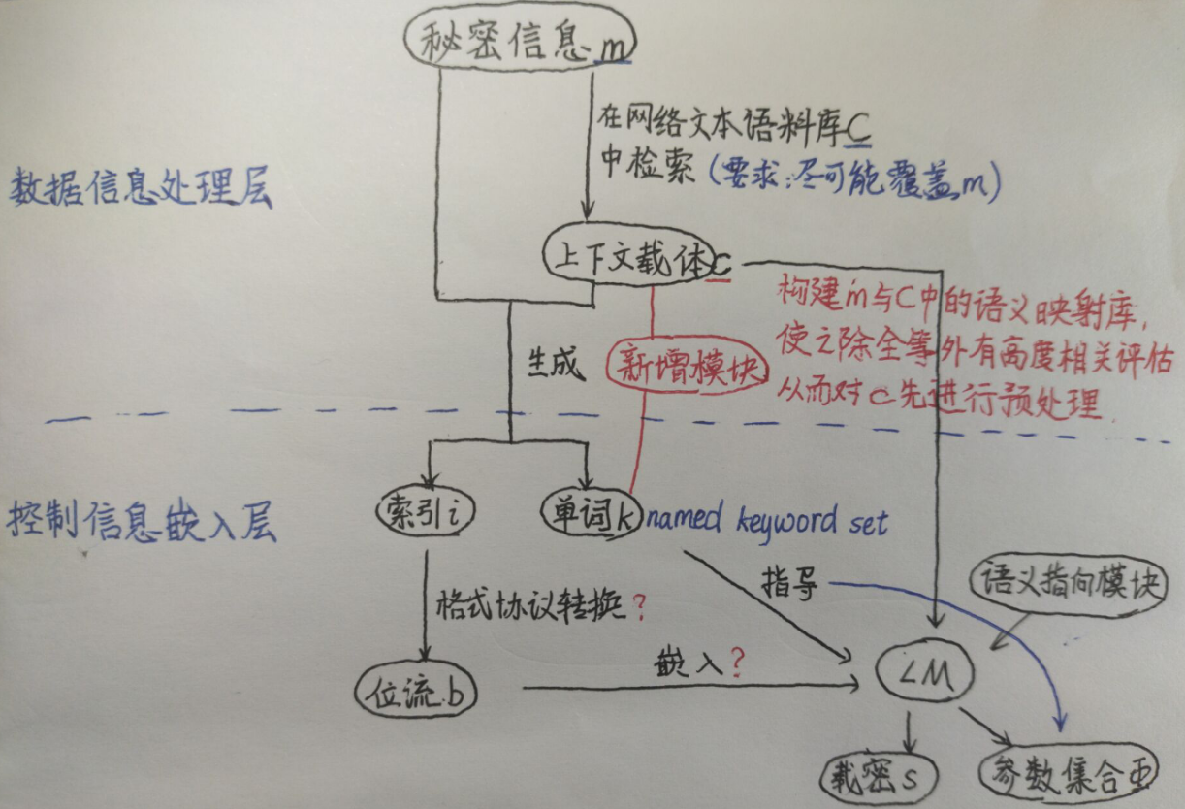
\includegraphics[width=11cm]{Hi-stega框架.png}
          \bottomcaption{\xiaowuhao{Hi-stega框架}}
      \end{figure}

    \subsection{预期目标}
      为了获取具有一定相关性的使用到的数据集为新闻数据集,将新闻的标题作为将要隐写的密文,将新闻的所有段落的内容作为
      信息隐写语料库C,最终实现将新闻的标题嵌入到新闻的段落中的一个文本隐写。
      
    \subsection{小组成员及分工}
      \subsubsection{张斌龙}
        主要负责部分代码的注释分析,以及代码的修正运行,部分数据的简单提取函数编写。
      \subsubsection{赵伯俣}
        主要负责utility相关提取关键词代码的注释分析、实验报告编写
      \subsubsection{刘竞优}
        encoder,decoder相关编码解码方法分析、答辩ppt制作

\section{相关背景}
\setlength{\parindent}{2em}
  在信息隐藏领域,现在已经发展出了诸如以图像、音频、视频、文本等一些媒体形式作为载体的隐写方法,
  但是受传输通道的影响,图像、音频、视频等一些媒体形式的载体在传输过程中可能会失真或者受到噪声影响,
  在各种载体中,文本隐写术受传输渠道影响较小,具有较高的鲁棒性和实用性,特别适合社交网络场景。\par
  目前为止较为热门的文本隐写方法有三种,分别为基于修改的方法、基于检索的方法和基于生成的方法。\par
  基于修改的方法\cite{ref2}通过词汇修改文本内容来嵌入信息。这些方法通常具有较低的嵌入率并且倾向于改变词频,这使得它们更容易受到隐写分析技术的影响。\par
  基于检索的方法\cite{ref3}首先对文本语料库中的样本进行编码,然后通过将样本与秘密消息映射来选择相应的句子进行传输。
  这些方法需要对文本语料库进行编码和构建,容量相对较低。然而,由于文本载体本身没有改变,基于检索的方法很难被现有的隐写分析方法检测到。\par
  使用神经网络生成文本\cite{ref4}。这些方法可以在一定程度上改善嵌入有效负载,但生成的文本在语义上是随机的,
  导致对某些隐写分析方法无效。基于生成的方法的灵活性,包括适应任何上下文和任何场景的能力,尚未得到充分探索和利用。\par
  文本隐写领域中,目前为止较为新颖的研究框架是使用Hi-stega进行文本隐写。

\section{项目内容}
  \subsection{主要框架}
        实现Hi-Stega层次隐写方法的主要程序伪代码如下所示
        \begin{algorithm}
            \caption{秘密信息嵌入算法}
            \begin{algorithmic}[1]  %每行显示行号
                \Require 某个输入秘密消息m、社交网络文本语料库C、语言模型LM
                \Ensure 隐写文本stego、隐写参数$\phi $

                \Function {DataInformationProcessing} {m,c}
                    \State 在C中检索,找到c可以覆盖m中尽可能多的单词;
                    \State 在c中记录这些词的索引i = (i1,i2,...,ip);
                    \If{$m_i \in m \ and \ m_i \notin c$}
                        \State {将 mi 添加到关键字集 k\;}
                    \EndIf 
                    \State \Return 控制信息k、i和数据载体c
                \EndFunction

                \Function {Control Information Embedding} {k,i,c}
                    \State 通过格式协议将i转换为比特流b
                     \While{生成过程并未结束}
                        \State {$W_{j} \gets LM(c,k,b)$}
                        \If{$w_j \in k$}
                            \State 从k中移除$w_{j}$
                            \State 将索引j添加到参数集Φ中;
                        \EndIf
                     \EndWhile
                    \State \Return 隐写文本stego、隐写参数$\phi $

                \EndFunction
            \end{algorithmic}
        \end{algorithm}

    \subsection{数据预处理}
      \subsubsection{数据清洗}
        由于原始数据集中并不是所有的字段在实验中都需要,所以需要对原始数据集进行清洗和预处理等工作。
        通过调用TweetClean.py代码、checker函数对数据中存在的表情符号进行情感分析、缩写词进行同义展开、
        与语义无关的字符的删除等数据清洗工作,方便模型进行识别与读取

      \subsubsection{提取主体数据字典}
        该部分的功能在news\_Search.py中进行实现,主要是将经过清洗之后的原始数据集test.data中存在的标题数据
        以及相关的内容进行提取,得到test\_title.txt文件。从而获得到将要隐写到载体中的密文信息
        然后需要对原始数据集中需要用到的数据进行筛选与提取,将提取得到的各项参数以jsonl格式保存到\\
        test\_data\_clean\_for\_test\_all.jsonl文件中。\par
        在本次实验中原作者给定的数据集有三个,复现过程中为了节省时间采用了较小的一个test.data文件进行训练。

      \subsubsection{数据提取结果}
        在运行预处理程序的过程中会出现由于数据集中混杂了一些其他编码的数据,导致分词时代码会报错,
        报错信息如下图所示
        \begin{figure}[H]
          \centering
          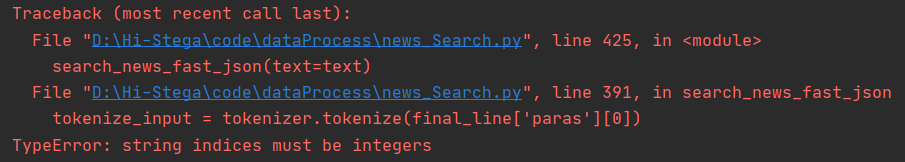
\includegraphics[width=13cm]{预处理报错.png}
          \bottomcaption{\xiaowuhao{预处理过程报错信息}}
        \end{figure}
        因为不是正常的字符。所以我们的处理只能是裁剪原始数据集。\par
        在本次实验中所使用的原始数据集的结构如下图所示
        \begin{figure}[H]
            \centering
            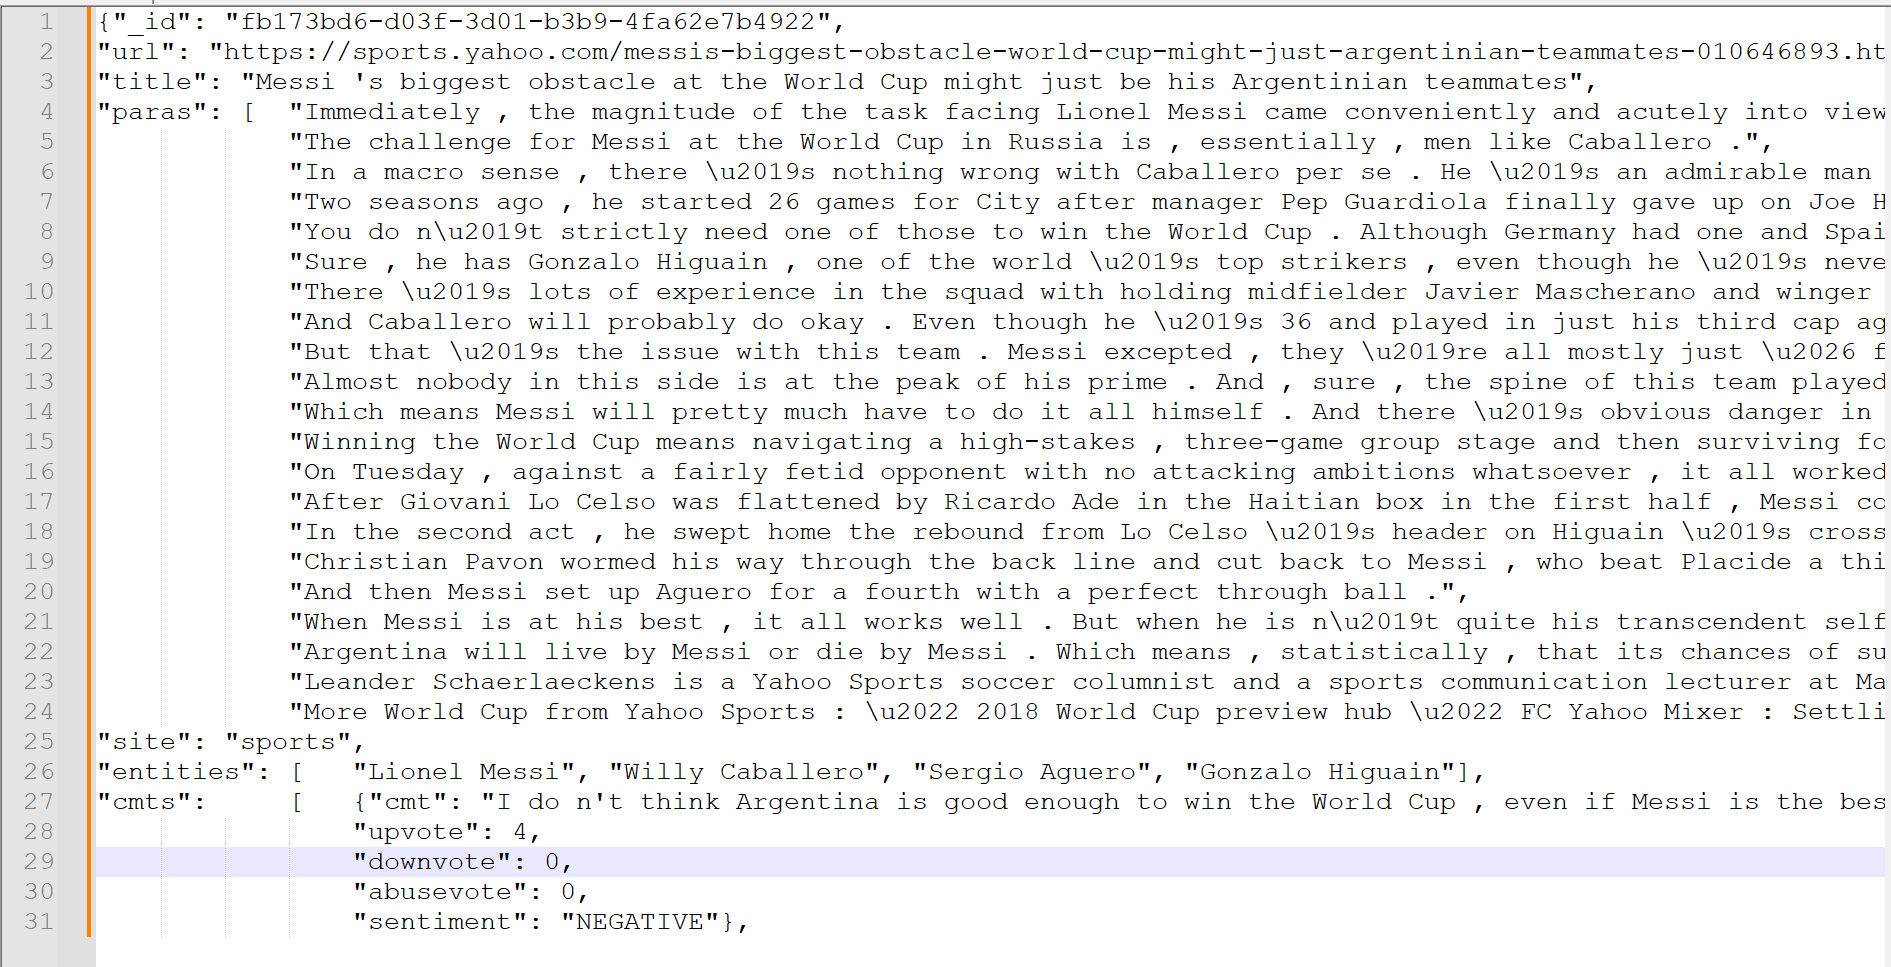
\includegraphics[width=13cm]{原始数据集.png}
            \bottomcaption{\xiaowuhao{原始数据集结构}}
        \end{figure}

        原始数据集中单项的数据结构如下表所示:
        \begin{table}[H]
            \caption{原始数据集结构}\label{tab1}
              \centering
            \begin{tabular*}{0.75\textwidth}{@{\extracolsep{\fill}}lc}
                \toprule
                数据集字段           &含义                                \\
                \midrule
                id           &唯一标识符\\
                url         &新闻来源的网址\\
                title       & 新闻标题\\
                paras       &新闻文章段落数组\\
                site        &新闻发布的网站或来源\\
                entities    &新闻中提到的主要实体\\
                cmts        &用户评论数组\\
                \bottomrule
            \end{tabular*}
        \end{table}        

        经过数据清洗和关键数据的提取操作之后得到的数据字典结果如下图所示
        \begin{figure}[H]
          \centering
          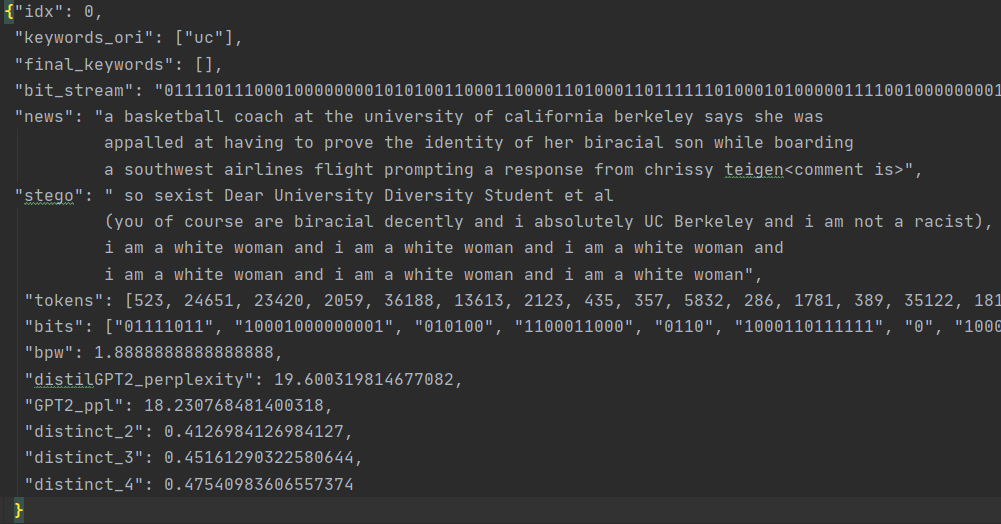
\includegraphics[width=13cm]{预处理结果.png}
          \bottomcaption{\xiaowuhao{预处理结果}}
        \end{figure}
        
    \subsection{构建keywords}
      因为在文本隐写过程中需要关键词来指导信息的隐写操作,在数据预处理步骤已经实现了对于原始数据集部分
      相关数据的提取,在构建keywords时调用get\_jsonl\_wo\_unk\_v3函数对数据集中提取出的关键词进行筛选
      并保存在新的jsonl文件中并且将关键词映射到对应嵌入向量后生成.pkl文件中。
      最后得到的关键词数据列表keyword\_sets如下图所示
      \begin{figure}[H]
        \centering
        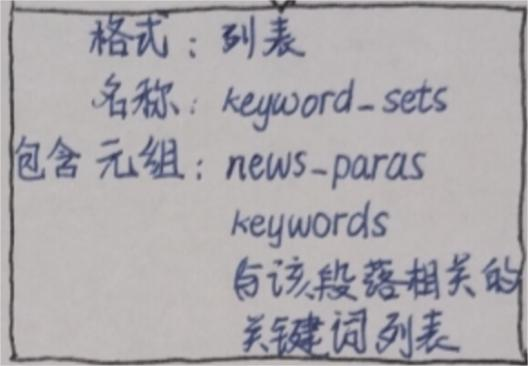
\includegraphics[width=6cm]{关键词数据.jpg}
        \bottomcaption{\xiaowuhao{关键词构建结果}}
      \end{figure}

    \subsection{构建模块}
      在隐写过程中需要使用到GPT-2模型进行构建,在使用大模型进行构建的过程中需要一定的语义指向模块,提示学习模块
      以及converter\_table\_glove.npy文件对于隐写生成结果进行指导。\par
      首先需要经过coverter\_table\_glove函数将GPT-2词汇表中的单词转换为glove嵌入表示的转换表得到GPT-2生成的
      指导文件。\par
      语义指导模块kG的作用是通过调整$p_{\theta }$使得语义能够接近\par
      $k=\left \{k_{1},k_{2},k_{3},\dots ,k_{n}  \right \} $\par
      提示学习模块prompt在GPT-2模型控制生成文本的过程中也会起到知道模型生成的文本更加流畅的功能。
        
    \subsection{隐写核心}
      在本次实验中所使用的隐写框架为首先根据秘密信息在文本语料库中选取与秘密信息最契合的文本作为隐写的载体信息,
      然后根据秘密信息在上下文载体中的存在与否来生成单词数组keyword\_set和索引i,然后将索引i的格式转换为比特流
      保存到变量bit\_stream中,将得到的比特流和经过编解码器编码后的单词数组传递给GPT-2模型即可生成出载密S以及参数集合体$\varphi $
      
    \subsection{结果评估}

      \subsubsection{计算相似度}
        该部分主要调用get\_sim函数来完成,该函数接收编码后的关键词的列表以及GPT模型生成的关键词列表
        以及数据预处理步骤中得到的呃转换表,以及一系列的参数之后计算输入的两组关键词之间的相似度
        最后将计算得到的相似度的值保存到sim中进行返回

      \subsubsection{评估文本质量}
        因为需要判断GPT模型生成的句子的质量来修改构建的指导模块,所以需要对于文本进行评价,通过
        调用evaluate\_quality系列函数,设 sequence 为文本序列,word 为特定单词,perplexity 为文本复杂度,
        guide 为布尔值,temp 为温度参数。\par
        评估文本质量的原理为:\par
        
        计算可以得到的质量分数\par
        $ Q = \frac{1}{\text{temp}} \cdot \exp ( - (w_1 \cdot \text{word\_count} + w\_3 \cdot \text{perplexity} ) ) $\par
        若采用线性方式对文本质量进行评估,perp为布尔值。其原理为:\par
        $Q_{\text{linear}} = \frac{1}{\text{temp}} \cdot \left( \text{word\_count} \pm w_3 \cdot \text{perplexity} \right)$
        通过这种评估质量的算法可以准确的指导GPT模型生成质量更加高的文本

      \subsubsection{计算句子困惑度}
        为了评价生成模型的质量,需要衡量语言模型性能的指标,衡量模型对测试数据的预测能力。\par
        在本次实验中采用的计算句子困惑度的数学方法为:\par
        $\text{PPL}(S) = \exp\left( \frac{1}{N} \sum_{i=1}^{n} \text{NLL}(s_i) \right)$
        根据产生的结果判断每个使用的模型的预测能力。较低的困惑度通常意味着模型对数据有更好的预测能力

      \subsubsection{计算平均比特数}
        在实验过程中,因为需要对隐写后的信息进行编码处理,所以应当计算隐写后stegos中tokens的平均比特数来评价
        不同的编码方式的效果。在本次实验中调用bpw系列函数计算平均比特数从而得到信息编码效率来评价不同的编码方式

      \subsubsection{计算文本多样性}
        使用大模型生成的文本可能具有语言结构和内容上比较单一的特性,因此需要对生成的结果计算多样性,
        在本次实验中调用distinct\_n函数对文本的多样性进行计算:\par
        定义n-gram的集合 G 为从文本example 中生成的所有n-gram的集合。对于给定的n,n-gram可以定义为:\par
        $G=\left \{ (x_{i},x_{i+1},\dots ,x_{i+n-1})\mid x_{i}\in example, 1\le i \le (len(example)-n+1)\right \} $\par
        然后对于每一个n-gram 都有$g\in G$,更新不同n-gram的数量 $n_{distinct}$和总的n-gram数量$n_{total}$这
        可以表示为\par
        $n_{distinct}=\left | \left \{ g\mid g\in G,count(g)=1 \right \}  \right | $\par
        $n_{total}=\sum_{g\in G}^{} count(g)$

\section{项目成果}
\setlength{\parindent}{2em}
  
  \subsection{最终成果}
    运行程序对yahoo新闻\cite{ref5}中得到的数据集进行隐写操作,为了保证隐写信息和载体的高度相关性,采用将新闻的标题隐写到文本中的方法,最终得到的隐写结果
    如下图所示    
    \begin{figure}[H]
      \centering
      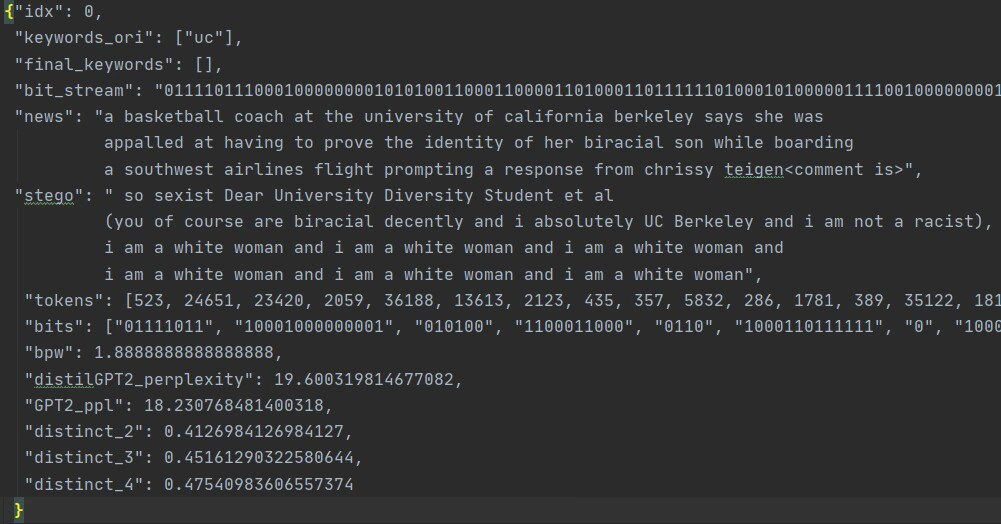
\includegraphics[width=13cm]{最终结果1.png}
      \bottomcaption{\xiaowuhao{隐写结果}}
    \end{figure}
    该结果使用传统的基于生成的方法进行隐写操作,将keyword作为大模型隐写的参考对象之一,
    使GPT模型依照keyword和一个随机生成的比特流序列以及一系列的语义指导模块进行隐写文本的生成\par
    在使用本次实验中设计的HiStega模型进行隐写后得到的结果如下图所示
    \begin{figure}[H]
      \centering
      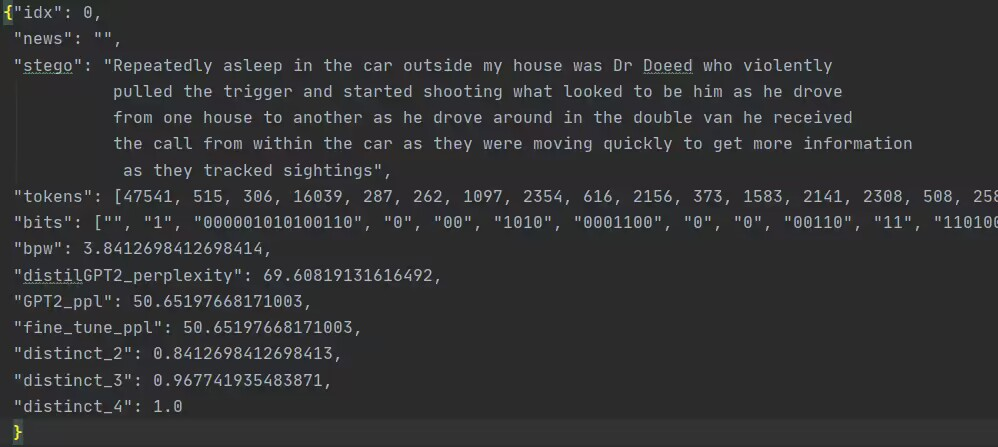
\includegraphics[width=13cm]{最终结果2.png}
      \bottomcaption{\xiaowuhao{隐写结果}}
    \end{figure}
    观察该结果可以发现生成的语句较为通顺,在其中也包含有一定的关键词信息,直接观察可以看出,本次实验中所采用的模型相较于传统的文本生成隐写模型
    有较大的优化

  \subsection{代码结构}
    本次实验中采用的一些主体功能代码如下图所示,该代码包含了模型框架隐写过程的整个流程,以及所有的功能代码
    并且包含部分隐写方式的运行脚本
    \begin{figure}[H]
      \centering
      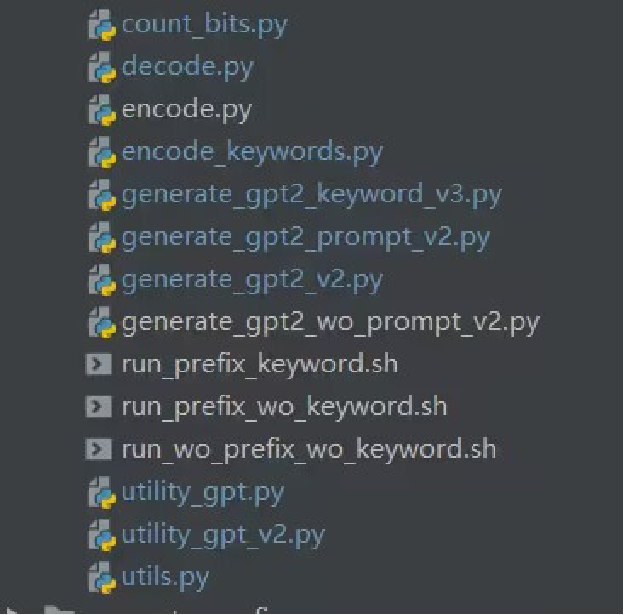
\includegraphics[width=9cm]{代码结构1.png}
      \bottomcaption{\xiaowuhao{代码结构}}
    \end{figure}

    本次实验中所采用的数据集文件以及数据集经过预处理过程产生的中间结果文件如下图所示,
    其中也包括因为未知原作者对数据集的处理方式而自己编写的数据预处理程序
    \begin{figure}[H]
      \centering
      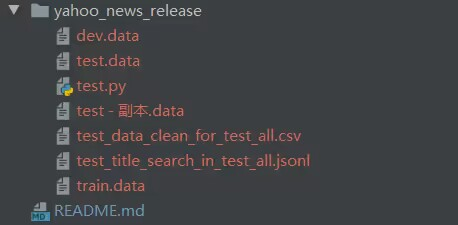
\includegraphics[width=9cm]{代码结构2.png}
      \bottomcaption{\xiaowuhao{代码结构}}
    \end{figure}

    本次实验中所使用到的一些依赖文件保存到了/data目录下,其中预处理所用到的程序代码和文件保存到/dataProcess下
    配置文件保存到/generate\_configs目录下;生成的结果保存到了generate\_keyword+num\_bit\_len\_bit目录下
    只使用GPT-2模型进行隐写文本生成的结果保存到了generate\_result目录下;实验中用来观察隐写过程
    并调试的日志文件存放到log\_prompt下。具体的目录结构如下图所示
    \begin{figure}[H]
      \begin{minipage}[t]{0.45\linewidth}
          \centering
          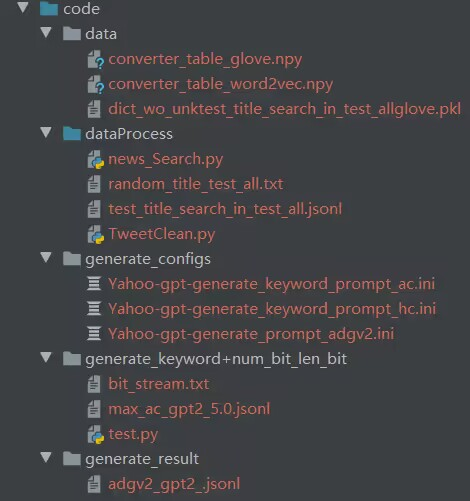
\includegraphics[width=5.5cm,height=6cm]{代码结构3.png}
      \end{minipage}
      \begin{minipage}[t]{0.45\linewidth}        %图片占用一行宽度的45%
          \hspace{10pt}
          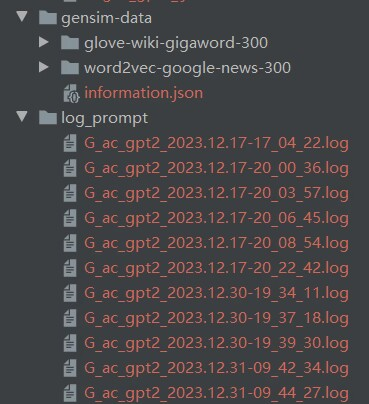
\includegraphics[width=5.5cm,height=6cm]{代码结构4.png}
      \end{minipage}
    \end{figure}

    由于附上源码时并不像破坏整个目录结构的完整性,但整个文件过大,所以做了如下操作:\par
    1.将Hi-Stega/yahoo\_news\_release中的dev.data和train.data删除\par
    2.将Hi-Stega/code/ginsim-data中两个词汇转换表中内容清空,因为运行代码能拉取\par
    这些改动不会影响代码运行,目的是为了减少压缩包的大小,因为这些表项都是大文件

  \subsection{性能评估}

    \subsubsection{预期目标}
      在本次实验中希望达到的预期目标是选取一个秘密信息能够在文本语料库中选取一个载体对秘密信息进行嵌入操作,
      并且在得到嵌入后的信息之后也能够将嵌入后的信息提取出来,但是在复现的过程中由于在生成的文本中嵌入使用的是GloVe模型,
      所以在创建嵌入向量文件pkl时引入的也是GloVe模型,在提取过程中也使用该pkl文件。按理来说是个简单的逆向使用,
      但是实际上代码报错。查询原因无果后推测是我们在运行代码时可能漏执行了某些关键代码。其中.pkl文件是由encode\_keywords.py中
      create\_enc\_dict函数生成。在程序中出现的报错信息如下图所示
      \begin{figure}[H]
        \centering
        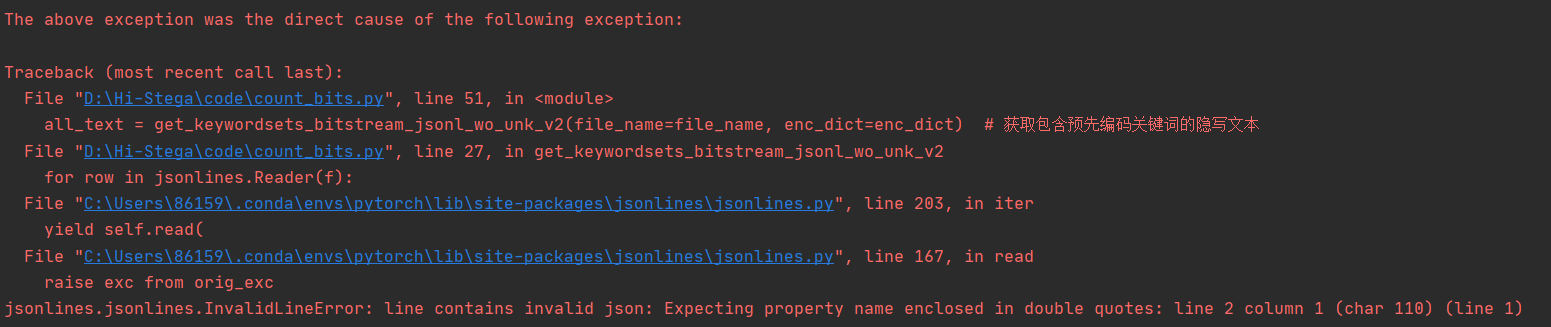
\includegraphics[width=13cm]{pkl解析报错.png}
        \bottomcaption{\xiaowuhao{pkl解析报错信息}}
      \end{figure}
      create\_enc\_dict函数的大致结构为创建字典映射从 CSV 文件中提取的关键词到它们在 GloVe 词嵌入(word embedding)中的向量表示。
      但是由于代码缺乏完整性,并且存在有众多未注释的不同版本的create\_enc\_dict系函数,所以导致在处理pkl文件时并不能
      对pkl文件进行正确的解析
  
    \subsubsection{编码方式}
      因为在信息隐写的过程的数据编码的方式也会对各个性能指标造成直接的影响,所以在本次实验中采用了霍夫曼编码HC\cite{ref6}、算术编码AC\cite{ref7}
      和自适应动态分组ADG\cite{ref8}三种编码方式使用相同的隐写算法进行信息隐写,计算隐写后文本的困惑度用于评价文本的流畅性,
      计算文本的多样性,得到的结果如下表所示
      \begin{table}[!h!tbp]
        \caption{编码方式不同对结果影响}\label{tab2}
          \centering
        \begin{tabular*}{0.75\textwidth}{@{\extracolsep{\fill}}lcc}
            \toprule
            编码方式          &流畅性(文本困惑度)         &多样性         \\
            \midrule
            霍夫曼编码          &18.23     &0.45     \\
            算术编码          &20.44     &0.47     \\
            自适应动态分组          &19.32    &0.44     \\
            \bottomrule
        \end{tabular*}
      \end{table}
      通过比较得到的文本流畅性和多样性的评价指标可以发现,编码方式的不同确实会对文本困惑度和文本的多样性造成一定的影响,但是在数值上
      的影响并不大。在三种编码方式中算术编码的文本困惑度要高于其他两种编码方式也就是说其文本的流畅性较低,但其多样性数值相较于其他
      两种编码方式较高。\par
      由此可见霍夫曼编码的文本困惑度最低即其文本的流畅程度很高,且其多样性也处在较高水平;算术编码的流畅性最低,但是其多样性在
      三种编码方式中处于较高位置;自适应动态分组则介于二者之间。\par
      因此得出结论,虽然三种不同的编码方式在流畅性和多样性上存在些许差别,但是差别的值较小,不会影响实验结果。

    \subsubsection{隐写方式}
      将程序运行得到的关于生成文本流畅性和多样性的数值统计得到的结果如下表所示
      \begin{table}[!h!tbp]
        \caption{隐写算法不同对结果影响}\label{tab3}
          \centering
        \begin{tabular*}{0.75\textwidth}{@{\extracolsep{\fill}}lccccc}
            \toprule
            隐写算法          &文本困惑度         &$distinct_{2}$ &$distinct_{3}$ &$distinct_{4}$   &bpw       \\
            \midrule
            传统隐写          &18.23     &0.41  &0.45    &0.47 &1.88     \\
            HiStega隐写          &50.65     &0.84  &0.96  &1.0  &3.84 \\
            \bottomrule
        \end{tabular*}
      \end{table}
      观察生成的结果可以看出,采用HiStage模型生成的隐写后的文本的文本困惑度较高,文本更加流畅,并且该模型生成的文本三次计算多样性也
      处在一个较高的水平,该模型的编码效率明显高于传统的编码方式

\subsection{局限性}

  1.generate\_gpt2\_keyword\_v3.py应该生成的依赖的文件编码方式为AC,但是在后续generate\_gpt2\_v2.py生成隐写文本时使用ADG\_V2编码方式,
  最终产生意义不明的隐写文本。并且在程序运行的过程中还会出现有大量的报错信息如下图所示
  \begin{figure}[H]
    \centering
    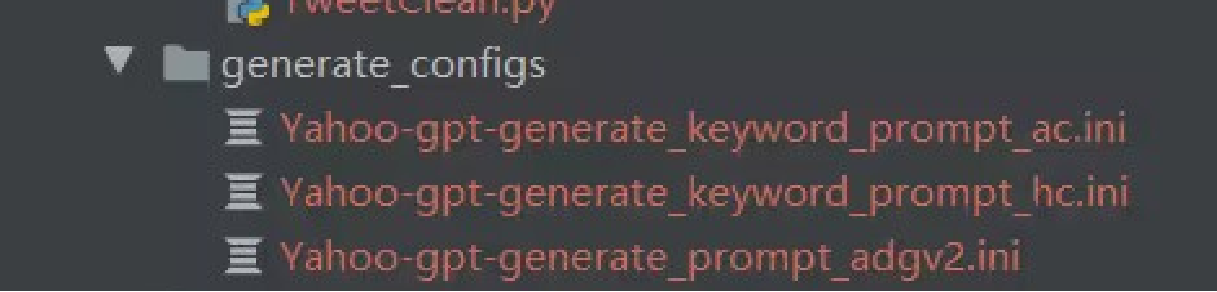
\includegraphics[width=13cm]{报错1.png}
    \bottomcaption{\xiaowuhao{报错信息}}
  \end{figure}\par

  2.源代码有大量注释代码段,同时没有明确的注释来说明这些代码段的作用,由此导致代码分析过程中有很多函数未被使用,
  这可能是导致实验结果不符合预期的部分原因。以下是utils.py文件中注释掉的部分代码。
  \begin{figure}[H]
    \centering
    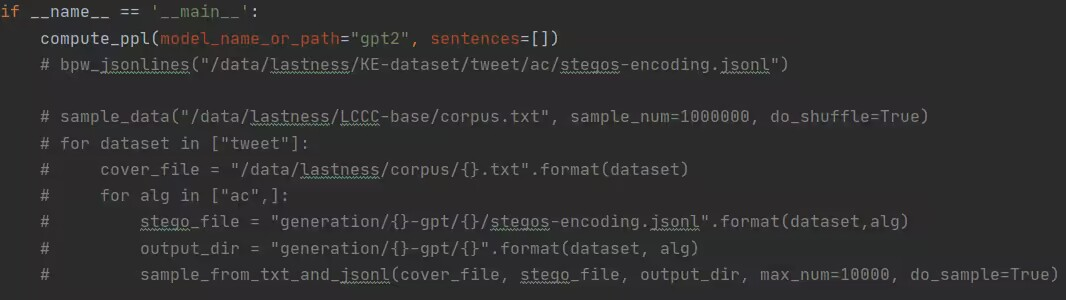
\includegraphics[width=13cm]{注释代码段.png}
    \bottomcaption{\xiaowuhao{大量注释代码段}}
  \end{figure}\par
  
  3.在运行generate系列函数中出现如下报错显示列表超过索引。这个报错的原因未知,按照道理在裁剪数据集后应该没有这样的错误,
  小组讨论后推测的结果可能是在预处理时得出的数据存在问题。
  \begin{figure}[H]
    \centering
    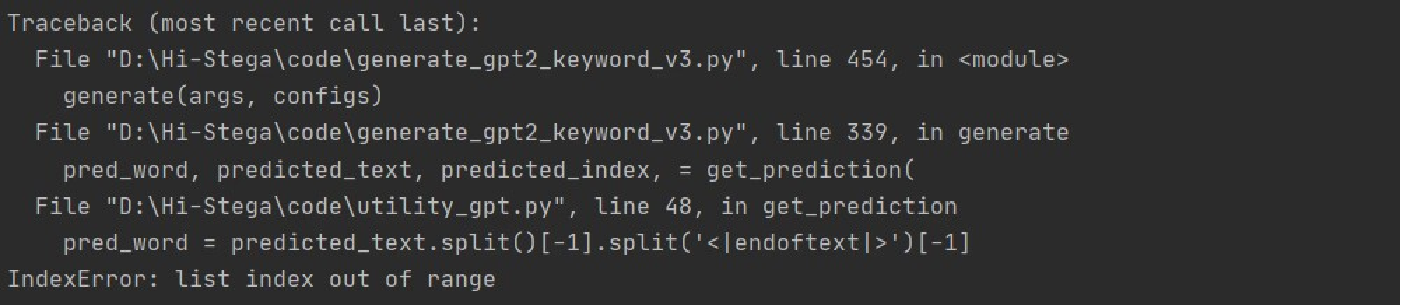
\includegraphics[width=13cm]{generate报错.png}
    \bottomcaption{\xiaowuhao{generate报错}}
  \end{figure}\par

  4.该模型的隐写过程非常依赖于文本语料库,如果能够有非常充足的文本语料库,那么隐写的结果将会非常好,但是在现实中并不存在无限大的并且存在与
  秘密信息匹配程度完美契合的文本作为载体,因此在实际隐写过程中会造成隐写结果并不理想的情况。\par
  5.在实验过程中因为时间有限,只采取了单个数据集进行信息隐写,并没有采用不同网络情境下的数据集进行多方位的测试,使得实验得出的结果可能存在
  片面的可能。\par
  6.同样因为实验时间有限,没有对该模型进行较为全面的隐写分析,没有针对该模型的抗隐写分析能力进行讨论和研究。

\section{总结及展望}

  \subsection{总结}
    在本次实验中,主要重心在于对于原始项目的复现上,并且由于论文较新所以原作者的实验代码并不全面造成复现中缺少关键步骤导致复现出的结果并不全面
  \subsection{展望}
    对关键词集K进行提前预处理,使得在隐写的过程中k的数据量能够更小,方便在嵌入模块中指导模型的嵌入,并且能够抵抗隐写分析\par
    对比特流生成和嵌入的过程进行更加有效的编码方式,使得模型的嵌入效率能够更高,使得模型具有更强的携带秘密信息的能力\par
    更换不同社会网络情境下的数据集,统计该模型在不同的数据集下的表现。\par
    对隐写模型进行多种隐写分析测试,分析该隐写模型的抗检测能力和鲁棒性

\newpage
\begin{thebibliography}{100} %引用上限为100篇

\bibitem{ref1}Wang H, Yang Z, Yang J, et al. Hi-Stega: A Hierarchical Linguistic Steganography Framework Combining Retrieval and Generation[C]//International Conference on Neural Information Processing. Singapore: Springer Nature Singapore, 2023: 41-54.
\bibitem{ref2}Chang, C.Y., Clark, S.: Practical linguistic steganography using contextual synonym substitution and a novel vertex coding method. Comput. Linguist. 40(2), 403–448 (2014)
\bibitem{ref3}Chen, X., Sun, H., Tobe, Y., Zhou, Z., Sun, X.: Coverless information hiding method based on the Chinese mathematical expression. In: Huang, Z., Sun, X., Luo, J., Wang, J. (eds.) ICCCS 2015. LNCS, vol. 9483, pp. 133–143. Springer, Cham (2015).
\bibitem{ref4}Xiang L, Wang R, Yang Z, et al. Generative Linguistic Steganography: A Comprehensive Review[J]. KSII Transactions on Internet \& Information Systems, 2022, 16(3). 

\bibitem{ref5}Yang, Z., Xu, C., Wu, W., Li, Z.: Read, attend and comment: a deep architecture for automatic news comment generation. In: Proceedings of the 2019 Conference on Empirical Methods in Natural Language Processing and the 9th International Joint Conference on Natural Language Processing (EMNLP-IJCNLP), pp. 50775089 (2019)

\bibitem{ref6}Yang, Z.L., Guo, X.Q., Chen, Z.M., Huang, Y.F., Zhang, Y.J.: RNN-Stega: linguistic steganography based on recurrent neural networks. IEEE Trans. Inf. Forensics Secur. 14(5), 1280–1295 (2018)
\bibitem{ref7}Ziegler, Z., Deng, Y., Rush, A.M.: Neural linguistic steganography. In: Proceedings of the 2019 Conference on Empirical Methods in Natural Language Processing and the 9th International Joint Conference on Natural Language Processing (EMNLPIJCNLP), pp. 1210–1215 (2019)
\bibitem{ref8}Zhang, S., Yang, Z., Yang, J., Huang, Y.: Provably secure generative linguistic steganography. In: Findings of the Association for Computational Linguistics: ACL-IJCNLP 2021, pp. 3046–3055 (2021)
\end{thebibliography}

\end{document}
    